\chapter{Common LaTeX Patterns}
\label{app:latex-patterns}

% This optional appendix is a compact cookbook, not part of the reachability
% argument. Keep only the patterns used by the thesis, replace every teaching
% asset, and discuss each retained figure, table, equation, or code listing in
% the surrounding prose.

\section{External illustration}

The project contains the original vector file used in
\cref{fig:external-illustration}. The explicit \texttt{.pdf} extension makes it
clear that this is an external asset loaded with \verb|\includegraphics| rather
than TikZ code inserted with \verb|\input|. PDF is preferable for diagrams and
plots; PNG or JPEG is appropriate for genuinely raster material.

\begin{figure}[htbp]
  \centering
  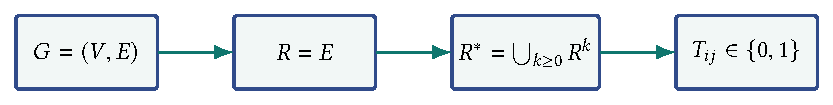
\includegraphics[width=0.82\linewidth]{figures/example-workflow.pdf}
  \caption{An original external PDF illustration of the example workflow.}
  \label{fig:external-illustration}
\end{figure}

% Replace both the file and caption. Record the source and licence for any
% non-original image, never stretch an image by setting incompatible width and
% height values, and inspect legibility at the final printed size.

\section{Multi-line and piecewise equations}

Use \texttt{align} when several displayed lines form one derivation and align at
a meaningful relation symbol. Label only lines cited later. For example,
\begin{align}
  T^{(0)}_{ij}
    &= A_{ij}\lor [i=j], \label{eq:pattern-initialisation}\\
  T^{(k)}_{ij}
    &= T^{(k-1)}_{ij}
       \lor\bigl(T^{(k-1)}_{ik}\land T^{(k-1)}_{kj}\bigr).
       \label{eq:pattern-update}
\end{align}
The update in \cref{eq:pattern-update} adds paths whose newest permitted
intermediate vertex is $k$.

A piecewise definition belongs inside a numbered equation when it must be
referenced:
\begin{equation}
  d(u,v)=
  \begin{cases}
    0, & u=v,\\
    \text{length of a shortest path}, & v\text{ is reachable from }u,\\
    +\infty, & \text{otherwise}.
  \end{cases}
  \label{eq:pattern-cases}
\end{equation}

\section{Text-rich table}

The \texttt{X} columns in \cref{tab:pattern-guide} share the available width and
wrap prose automatically. Use a normal \texttt{tabular} environment for compact
numeric data and introduce \texttt{longtable} only when a genuine table must
continue across pages, as shown next.

\begin{table}[htbp]
  \centering
  \caption{Choosing a compact table pattern.}
  \label{tab:pattern-guide}
  \begin{tabularx}{\linewidth}{@{}l>{\raggedright\arraybackslash}X>{\raggedright\arraybackslash}X@{}}
    \toprule
    Content & Recommended treatment & Common mistake \\
    \midrule
    Measurements & State units and uncertainty in headings or notes. & Repeating units in every cell. \\
    Long descriptions & Use a wrapping \texttt{X} column and concise prose. & Shrinking the entire table until text is unreadable. \\
    Many rows & Consider an appendix or a machine-readable companion file. & Splitting one logical row across pages manually. \\
    \bottomrule
  \end{tabularx}
\end{table}

\section{Table continuing across pages}

\texttt{longtable} lets one logical table break across pages. The caption and
the column headings are declared once, and the heading block is repeated on every
continuation page. \Cref{tab:pattern-checklist} shows the pattern with a
pre-submission checklist.

\begin{longtable}{@{}p{0.2\linewidth}p{0.62\linewidth}c@{}}
  \caption{A checklist typeset with \texttt{longtable}.}
  \label{tab:pattern-checklist}\\
  \toprule
  Area & Check & Done \\
  \midrule
  \endfirsthead
  \toprule
  Area & Check & Done \\
  \midrule
  \endhead
  \midrule
  \multicolumn{3}{r@{}}{\emph{Continued on the next page}}\\
  \endfoot
  \bottomrule
  \endlastfoot
  Metadata & Titles, author, supervisors, academic year, date, and keywords are correct. & $\square$ \\
  Language & The selected main document and the language of the PDF metadata agree. & $\square$ \\
  Comments & The advice comments (lines starting with \texttt{\%}) no longer describe the example. & $\square$ \\
  Cover & Logos, supervisors, academic referent, and laboratory are correct and authorised. & $\square$ \\
  Abstract & The abstract states the question, method, main result, and limitations. & $\square$ \\
  Contents & Every chapter and appendix appears with the right page number. & $\square$ \\
  Chapters & Example chapters are replaced and no unused chapter file is included. & $\square$ \\
  Figures & Each figure is cited, captioned below, and legible when printed. & $\square$ \\
  Tables & Each table is cited and captioned above, with units stated. & $\square$ \\
  Equations & Only equations cited later carry a label. & $\square$ \\
  Theorems & Statements are numbered by chapter, and each one is used or discussed. & $\square$ \\
  Bibliography & Every printed entry is cited; DOIs and years have been checked. & $\square$ \\
  Links & Cross-references and citations resolve, and no reference is left undefined. & $\square$ \\
  Build & A clean full compile reports no missing file and no overfull box. & $\square$ \\
  PDF & Fonts are embedded and every page has been inspected. & $\square$ \\
  Submission & The final PDF follows the programme and supervisor instructions. & $\square$ \\
\end{longtable}

% Replace the rows with your own table. Keep the caption above the table, keep
% \endfirsthead and \endhead identical in their column structure, and avoid
% longtable for tables that fit comfortably on one page.

\clearpage
\section{Code listing}

The portable \texttt{listings} package used by \cref{lst:graph-traversal}
requires no shell escape; syntax colouring is intentionally restrained.

% For a long program, keep it in its own file and load it with
% \lstinputlisting[style=TemplateCode,language=Python]{code/my-program.py}
\begin{lstlisting}[
  style=TemplateCode,
  language=Python,
  caption={A short graph traversal.},
  label={lst:graph-traversal}
]
def reachable(graph, source):
    seen = {source}
    frontier = [source]
    while frontier:
        vertex = frontier.pop()
        for neighbor in graph.get(vertex, []):
            if neighbor not in seen:
                seen.add(neighbor)
                frontier.append(neighbor)
    return seen
\end{lstlisting}

Together, \cref{fig:external-illustration,eq:pattern-cases,tab:pattern-guide,lst:graph-traversal}
show the recommended cycle: introduce an object, present it, assign a stable
label, and interpret it in the text.
